%++++++++++++++++++++++++++++++++++++++++
% Don't modify this section unless you know what you're doing!
\documentclass[a4paper,12pt]{article}
\usepackage{listings} % code blocks
\usepackage{tabularx} % extra features for tabular environment
\usepackage{amsmath}  % improve math presentation
\usepackage{graphicx} % takes care of graphic including machinery
\usepackage{subcaption} % necessary for subfigures
\usepackage{float}
\usepackage[margin=3.0cm,a4paper]{geometry} % decreases margins
%\usepackage{cite} % takes care of citations
%\usepackage[final]{hyperref} % adds hyper links inside the generated pdf file
%++++++++++++++++++++++++++++++++++++++++

\setlength{\parindent}{0pt}
\usepackage{hyperref}

\begin{document}

\title{Deep Learning Lab \\ Exercise 03 }
\author{Megan Klaiber}
\date{\today}
\maketitle

\section{Introduction}

In this exercise a behavioral cloning agent will be implemented and its performance will be evaluated on the CarRacing control task of OpenAi Gym. Therefore data were collected by driving on the track. For training 45000 samples were used and for testing 5000.

The distribution of actions in the dataset ist imbalanced. To avoid problems with that during training the actions were uniformly sampled.


\section{First Agent}\label{first}
For the first try the architecture of the last exercise were used. So it is a CNN with two convolutional layers with 16 5x5 filters, each followed by a Relu activation function and a max pooling layer of size 2. A fully connected succeed with 128 units and a softmax layer is used subsequent. The network is optimized with cross-entropy loss and stochastic gradient descent.
It was trained over 1000 minibatches each of size 64. Learning rate was 0.0001 and the input was only the current image.

In \autoref{fig:uniform} you can see the validation and train error with this architecture. This doesn't look so bad but the evaluation of the performance over 15 test episodes isn't so good. \autoref{tab:uniform} shows the mean achieved reward and the standard deviation of the evaluation. \\

%mean: - 57.46
%std: 52.94

\begin{table}[h] 
	\centering
	\begin{tabular}{|c | c|} 
		\hline
		\bfseries{REWARD} & \bfseries{STD} \\ 
		\hline
		- 57.46 & 52.94 \\  
		\hline
	\end{tabular}
	\caption{\label{tab:uniform} Mean reward and standard deviation.}
\end{table}


\begin{figure}[H]
	\centering 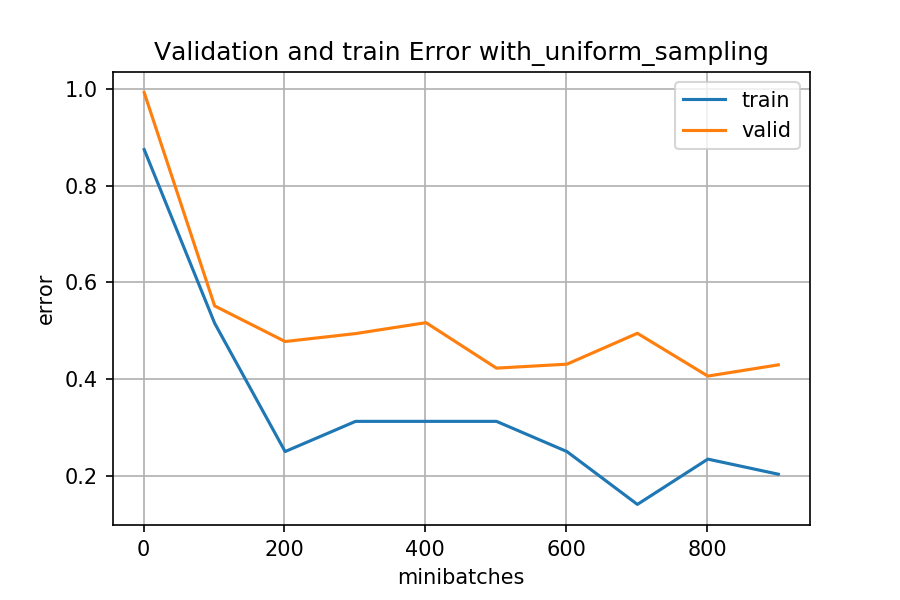
\includegraphics[width=11.70cm, height=7.9cm]{plots/valid_error_with_uniform_sampling.png}
	\caption{
		\label{fig:uniform}
		Change of validation and train error during 1000 training minibatches and first architecture.
	}
\end{figure}

\section{Improved Agent}\label{improved}
To improve the bad result of \autoref{first} another architecture is tested. This CNN has four convolutional layer with 76 filters and ReLu activation function. Then three fully connected layer and an output layer follow. The network is optimized with mean squarred error and Adam optimizer. It was trained over 1000 minibatches each of size 64. Learning rate was 0.0003 and the input was only the current image. 

In \autoref{fig:improved} you see the validation and train error with this architecture. Here the validation error isn't that good. But if you have a look at \autoref{tab:improved} you see that the agent can achieve a much better result during evaluation than the first agent in \autoref{first}.

So if you leave the max pooling layer off and increase the filter size you do better in this task. Important information about the state get lost through pooling layer and in the task of CarRacing this has a bad impact on learning. In addition more details can be learned during training with a higher number of filters. Also the Adam optimizer seems more stable than the stochastic gradient descent.\\


\begin{table}[h] 
	\centering
	\begin{tabular}{|c | c|} 
		\hline
		\bfseries{REWARD} & \bfseries{STD} \\ 
		\hline
		501.99 & 316.34 \\  
		\hline
	\end{tabular}
	\caption{\label{tab:improved} Mean reward and standard deviation.}
\end{table}



\begin{figure}[H]
	\centering 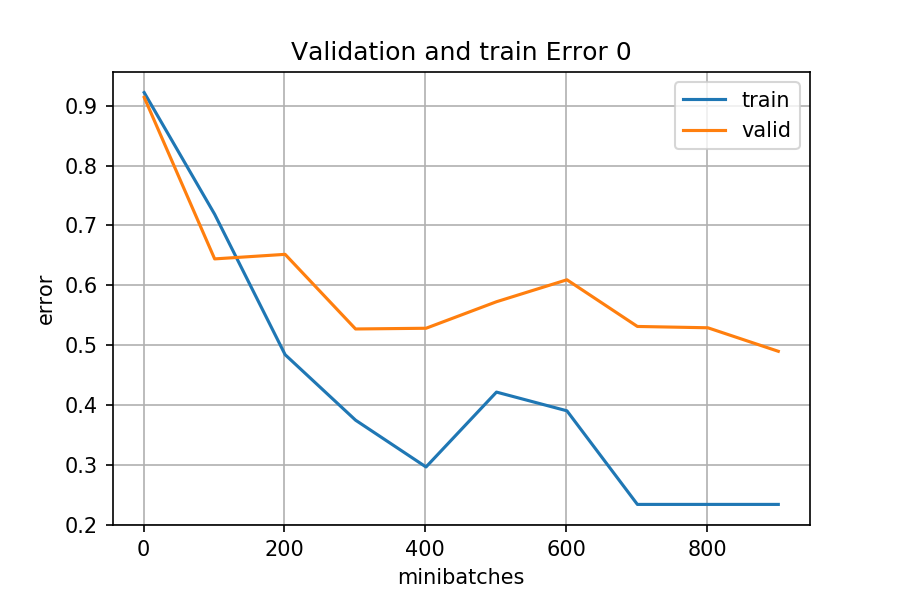
\includegraphics[width=11.70cm, height=7.9cm]{plots/valid_error_0.png}
	\caption{
		\label{fig:improved}
		Change of validation and train error during 1000 training minibatches and improved architecture.
	}
\end{figure}

This architecture is used in the following experiments.


\section{Impact of Batch Size}\label{batch}
In this experiment the batch size is evaluated. So the batch size represent the number of demonstrations during training. The following values are tested: \{32, 64, 128\}

In \autoref{fig:batch} you see the validation error during training and with the different batch sizes. Here the highest value achieve the lower validation error. Also during 15 test episodes (\autoref{tab:batch}) the model trained with the highest batch size get the best result. This is the impact of the higher number of demonstrations. So the result of batch size = 64 should be higher than the one of batch size = 32.


\begin{table}[h] 
	\centering
	\begin{tabular}{|c |c | c|} 
		\hline
		\bfseries{BATCH SIZE} & \bfseries{REWARD} & \bfseries{STD} \\ 
		\hline\hline
		32 & 754.81 & 124.57\\ 
		
		64 & 501.99 & 316.34 \\
		
		128 & 835.65 & 115.88 \\ 
		\hline
	\end{tabular}
	\caption{\label{tab:batch} Mean reward and standard deviation.}
\end{table}

\begin{figure}[H]
	\centering 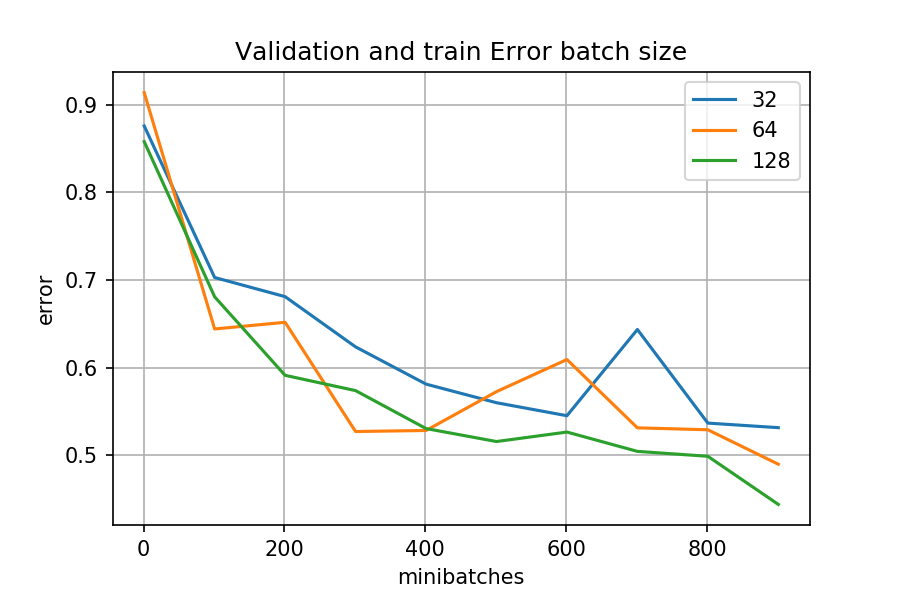
\includegraphics[width=11.70cm, height=7.9cm]{plots/valid_error_batch.png}
	\caption{
		\label{fig:batch}
		Change of validation and train error during 1000 training minibatches and batch size of 32, 64 and 128.
	}
\end{figure}

\section{Impact of History length}\label{history}

In this experiment the history length of the input is evaluated. This means that the history of the last images are append to the input. The following values are tested: \{1, 3, 5\}

In \autoref{fig:hist} you see the validation error during training and with the different history lengths. Here the highest length has the lowest validation error. If you compare this to the results of the testing episodes in \autoref{tab:hist} you see that here the highest lenght achieve the worst result. It was expected that the results with higher history length are better.


\begin{table}[h] 
	\centering
	\begin{tabular}{|c |c | c|} 
		\hline
		\bfseries{HISTORY LENGTH} & \bfseries{REWARD} & \bfseries{STD} \\ 
		\hline\hline
		1 & 804.03 & 127.49 \\ 
		
		3 & 503.55 & 165.58\\
		
		5 & 391.83 & 271.65\\ 
		\hline
	\end{tabular}
	\caption{\label{tab:hist} Mean reward and standard deviation.}
\end{table}

\begin{figure}[H]
	\centering 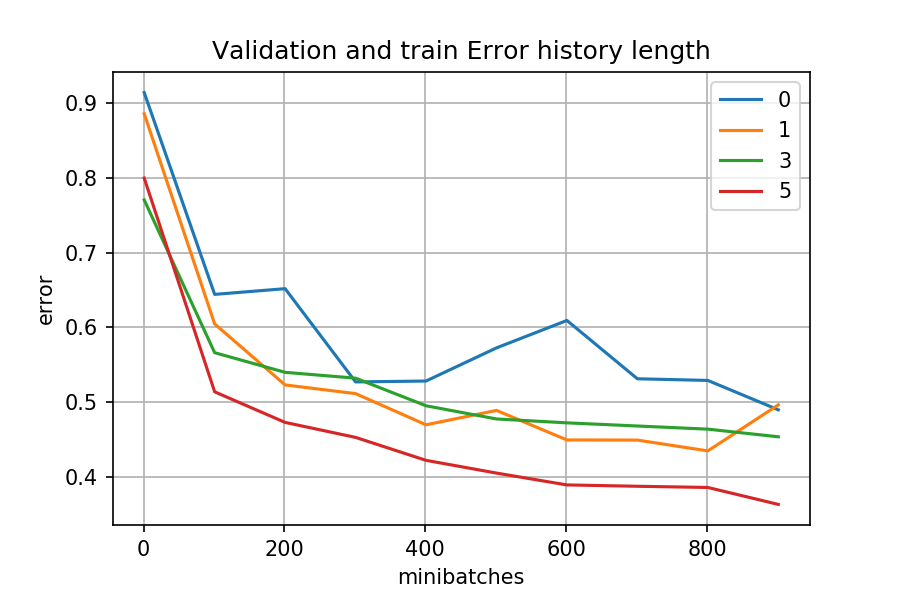
\includegraphics[width=11.70cm, height=7.9cm]{plots/valid_error_hist.png}
	\caption{
		\label{fig:hist}
		Change of validation and train error during 1000 training minibatches and history lenght of 0, 1, 3 and 5.
	}
\end{figure}



\section{Conclusion}
With this exercise you see that it is important to adjust the architecture individually to the given task. Also the hyperparameter tuning is important and you see that every hyperparameter has their individually impact on the training.

%\begin{itemize}
%	\item learning rate: 0.15
%	\item epochs: 30
%	\item batch size: 30
%	\item optimizer: stochastic gradient descent
%\end{itemize}

%\autoref{fig:train_valid_error}


\end{document}
